\question[6]
Bestimme für den Graphen einen minimalen Spannbaum mit dem Algorithmus von Kruskal. Immer wenn der Algorithmus uns eine
Wahl lässt, wählen wir in alphabetischer Reihenfolge. Für eine Kante nennen wir die Knoten ebenfalls
in alphabetischer Reihenfolge.

a. Gib die Kanten in der Reihenfolge an, in der sie gewählt werden.  \\
b. Gib die Kosten des MST an. \\
c. Zeichne des Chefbaum des einfachen Algorithmus nach dem Verfahren aus dem Unterricht. \\
d. Zeichen den optimierten Chefbaum des Algorithmus mit path-compression und union by rank
nach dem Verfahren aus dem Unterricht.

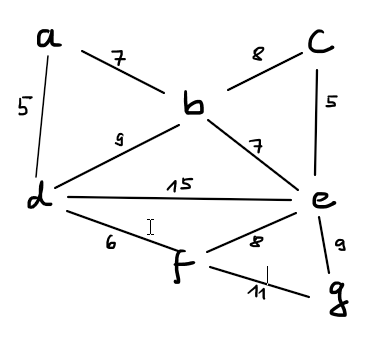
\includegraphics[height=3cm]{\pfad/Graphen/Aufgaben/kruskal_03/kruskal_03.png}
\begin{solutionbox}{9cm}
\begin{lstlisting}
a-d: 5   Chef von a wird d
c-e: 5   Chef von c wird e
d-f: 6   Chef von d wird f
a-b: 7   Chef von f wird b
b-e: 7   Chef von b wird e
e-g: 9   Chef von e wird g
Gesamtkosten:  39
\end{lstlisting}
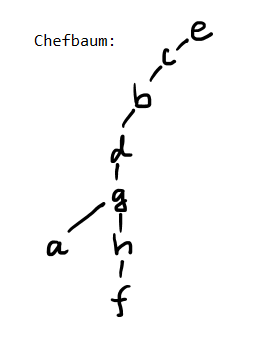
\includegraphics[height=5cm]{\pfad/Graphen/Aufgaben/kruskal_03/chefbaum.png}
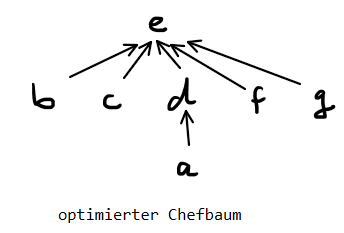
\includegraphics[height=3cm]{\pfad/Graphen/Aufgaben/kruskal_03/chefbaum_opt.png}
\end{solutionbox}
